\ExamPart{Câu trắc nghiệm nhiều phương án lựa chọn}{3}{Mỗi câu hỏi thí sinh chỉ chọn một phương án.}

\NQuestion Cho phương trình $x^2-8x+12=0$. Tổng hai nghiệm của phương trình bằng

\ChoicesOneLine{$8$.}{$12$.}{$-8$.}{$4$.}

\NQuestion Trong mặt phẳng tọa độ $Oxy$, cho vectơ $\vec u=(2;-5)$. Độ dài của vectơ $\vec u$ bằng

\ChoicesOneLine{$\sqrt{29}$.}{$7$.}{$\sqrt{21}$.}{$29$.}

\NQuestion Trong mặt phẳng tọa độ $Oxy$, phương trình tổng quát của đường thẳng đi qua điểm $A(2;3)$ và có vectơ pháp tuyến $\vec n=(1;-2)$ là

\ChoicesTwoLines
{$x-2y+4=0$.}
{$x+2y-8=0$.}
{$2x-y+1=0$.}
{$x-2y-4=0$.}

\NQuestion Cho đường tròn $(C):(x+1)^2+(y-4)^2=16$. Điểm nào sau đây là tâm của đường tròn?

\ChoicesOneLine{$(-1;4)$.}{$(1;-4)$.}{$(-1;-4)$.}{$(4;-1)$.}

\NQuestion Cho elip $(E):\dfrac{x^2}{36}+\dfrac{y^2}{16}=1$. Độ dài trục lớn của elip bằng

\ChoicesOneLine{$6$.}{$12$.}{$8$.}{$10$.}

\NQuestion Cho hàm số bậc hai $y=f\left(x\right)$ có đồ thị như hình dưới đây. Tập nghiệm của bất phương trình $f\left(x\right)\ge 0$ là

\begin{center}
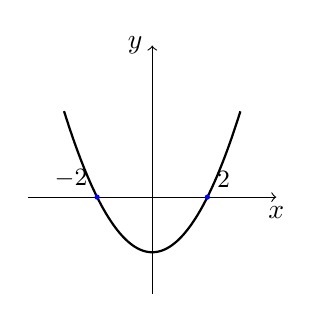
\begin{tikzpicture}[scale=0.35]
    \draw[->] (-4.5,0) -- (4.5,0) node[below] {$x$};
    \draw[->] (0,-3.5) -- (0,5.5) node[left] {$y$};

    \draw[thick, domain=-3.2:3.2, samples=200] plot (\x,{0.5*(\x*\x)-2});
    \draw[dashed] (-2,0) -- (-2,0);
    \draw[dashed] (2,0) -- (2,0);

    \fill[color=blue] (-2,0) circle (2.7pt);
    \fill[color=blue] (2,0) circle (2.7pt);
    \node[above left] at (-2,0) {\small $-2$};
    \node[above right] at (2,0) {\small $2$};
\end{tikzpicture}

\end{center}

\ChoicesTwoLines
{$(-\infty;-2]\cup[2;+\infty)$.}
{$[-2;2]$.}
{$(-2;2)$.}
{$(-\infty;-2)\cup(2;+\infty)$.}

\NQuestion Một biển quảng cáo hình chữ nhật có chiều dài hơn chiều rộng $3$m và diện tích bằng $54$m$^2$. Chiều rộng của biển quảng cáo là

\ChoicesOneLine{$6$m.}{$9$m.}{$3$m.}{$12$m.}

\NQuestion Từ các chữ số $0,1,2,3,4,5$, có thể lập được bao nhiêu số tự nhiên có $3$ chữ số khác nhau và chia hết cho $5$?

\ChoicesOneLine{$20$.}{$18$.}{$24$.}{$30$.}

\NQuestion Trong mặt phẳng tọa độ $Oxy$, cho hai điểm $A(-1;2)$, $B(3;2)$. Phương trình đường trung trực của đoạn thẳng $AB$ là

\ChoicesOneLine{$x=1$.}{$y=2$.}{$x=-1$.}{$y=1$.}

\NQuestion Một tam giác có đáy bằng $10$cm và chiều cao bằng $6$cm. Diện tích của tam giác đó bằng

\ChoicesOneLine{$16$cm$^2$.}{$30$cm$^2$.}{$60$cm$^2$.}{$32$cm$^2$.}
